\chapter{Metric Space}
\section{Definition}
\dfn{Metric Space $\bs{X}$}{A set $X$ with a function $d\:\ X\times X\to\bbR_{\geq 0}$ such that\begin{enumerate}[label=\bfseries\tiny\protect\circled{\small\arabic*}]
		\item $d(x,y)=0\iff x=y$
		\item $d(x,y)=d(y,x)$
		\item $d(x,z)\leq d(x,y)+d(y,z)$
	\end{enumerate}}
Notice that there is no homogeneity condition, and it does ot make sense as we don't have a field. In fact there is no notion of addition. But the condition \ref{n:1} of norm has to be satisfied by this distance. Also we don't have a translational condition i.e. distance between $x,y$ and distance  between $x+v,y+v$ has to be same. Hence
\begin{note}
	A metric space need not be a vector space. So it doesn't need a zero, or a notion of addition or scalar multiplication.
\end{note}
If I take a metric space and take any subset of it. And those three conditions of distance functions are still satisfied.
\begin{note}
	Any subset of metric space is a metric space under the same distance function.
\end{note}
\section{Open and Closed Ball and Set}
\dfn{Open Ball and Closed Ball in a Metric Space}{An open ball of radius $r$ with center $c\in X$ in a metric space $X$ is $$B_r(c)=\{x\in X\mid d(c,x)< r\}$$and a closed ball is $$\overline{B_r(c)}=\{x\in X\mid d(c,x)\leq r\}$$}
\pagebreak
\dfn{Open Set and Closed Ball in a Metric Space}{An open set in a metric space $X$ is one of the form of union of some open balls and a closed set in a metric space $X$ is one of the form of $X\setminus $some open sets}


\nt{We will do topology in Normed Linear Space  (Mainly $\bbR^n$ and occasionally $\bbC^n$)using the language of Metric Space}
\ex{Open Set and Close Set}{
	\begin{tabular}{rl}
		Open Set:   & $\bullet$ $\phi$                                              \\
		            & $\bullet$ $\bigcup\limits_{x\in X}B_r(x)$ (Any $r>0$ will do) \\[3mm]
		            & $\bullet$ $B_r(x)$ is open                                    \\
		Closed Set: & $\bullet$ $X,\ \phi$                                          \\
		            & $\bullet$ $\overline{B_r(x)}$                                 \\
		            & $x-$axis $\cup$ $y-$axis
	\end{tabular}}

\qs{}{Is the set ${x-}$axis${\setminus\{\text{Origin}\}}$ a closed set}\sol We have to take its complement and check whether that set is a open set i.e. if it is a union of open balls

Now this works well for points which are above or below the $x-$axis. But for origin no matter how small the ball we take it willl have points from $x-$axis. Hence the set is not a closed set.
\qs{}{Any continuous path in $\bbR^2$ is closed where $\text{path}=f:[0,1]\to\bbR^2$}
\sol This is true. To be proved later.\\
Analogous to: For continuous function $f:[0,1]\to\bbR$, the image is a closed interval
\qs{}{If i take $X=x-$axis $\cup\ y-$axis then is it open}
\sol Yes because here the space is only the union of those two axis. So any ball would be like a cross or line but it just as the metric space given to us. [It is open for this metric space but not open in $\bbR^2$]
\nt{If $S\subset X$, then $S$ itself has a collection of open sets of $S$ by containing $S$ as a metric space.}
\dfn{Neighborhood}{For a point $x$ in metric space $X$, a neighborhood of $x$ is a set $N$ such that $x\in $an open set $U\subset N$

	\vspace*{2mm}
	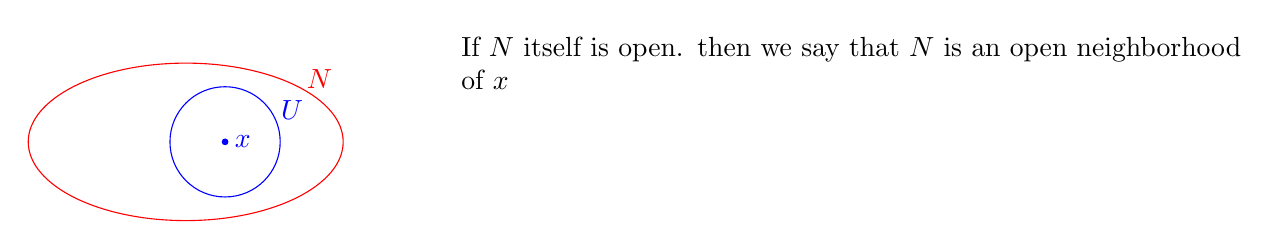
\begin{tikzpicture}
		\draw[red] (0.5,0) circle [x radius=2cm, y radius=1cm] ;
		\draw (2.2,0.8) node[red]{$N$};
		\draw [blue] (1,0) circle (7mm) ;
		\filldraw[blue] (1,0) circle (1pt) node[anchor=west]{$x$};
		\draw (1.85,0.4) node[blue]{$U$};
		\node[black,text width=10cm] at (9,1){If $N$ itself is open. then we say that $N$ is an open neighborhood of $x$};
	\end{tikzpicture}}


\thm{}{If $x\in$ open set $V$ then $\exists$ $\delta>0$ such that $B_{\delta}(x)\subset V$}

\begin{myproof}By openness of $V$, $x\in B_r(u)\subset V$
	\begin{center}
		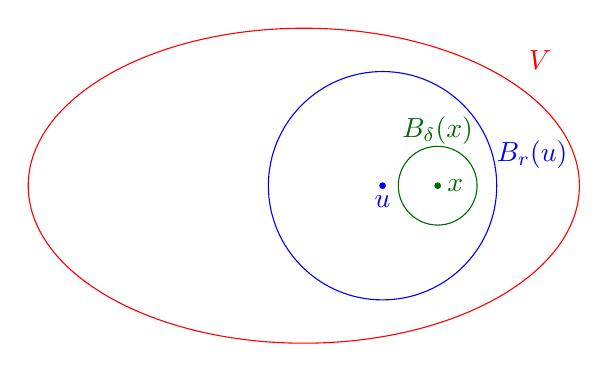
\begin{tikzpicture}
			\draw[red] (0,0) circle [x radius=3.5cm, y radius=2cm] ;
			\draw (3,1.6) node[red]{$V$};
			\draw [blue] (1,0) circle (1.45cm) ;
			\filldraw[blue] (1,0) circle (1pt) node[anchor=north]{$u$};
			\draw (2.9,0.4) node[blue]{$B_r(u)$};
			\draw [green!40!black] (1.7,0) circle (0.5cm) node [yshift=0.7cm]{$B_{\delta}(x)$} ;
			\filldraw[green!40!black] (1.7,0) circle (1pt) node[anchor=west]{$x$};
		\end{tikzpicture}
	\end{center}

	Given $x\in B_r(u)\subset V$, we want $\delta>0$ such that $x\in B_{\delta} (x)\subset B_r(u)\subset V$. Let $d=d(u,x)$. Choose $\delta $ such that $d+\delta<r$ (e.g. $\delta<\frac{r-d}{2}$)

	If $y\in B_{\delta}(x)$ we will be done by showing that $d(u,y)<r$ but $$d(u,y)\leq d(u,x)+d(x,y)<d+\delta<r$$
\end{myproof}
\nt{$V$ is open $\iff\bigcup\limits_{x\in V}B_r(x)$ (where $r$ depends on $x$)}
\thm{}{Let $X$ be a metric space.\begin{enumerate}
		\item Union of open sets is open
		\item Intersection of two open sets is open
	\end{enumerate}Analogues to these as we are just taking complement of the open sets
	\begin{enumerate}[label=\arabic*$'$.]
		\item Arbitrary intersection of closed sets is closed
		\item Finite union of closed sets is closed.
	\end{enumerate}

}

\begin{myproof}
	\begin{enumerate}
		\item Let $\{V_{\alpha}\}_{\alpha\in I}$ be a collection of open sets where $I$ is an index set. We want ti show $\bigcup\limits_{\alpha\in I}V_{\alpha}$ is open in $X$. Since each $V_{\alpha}$ is open $V_{\alpha}=\bigcup\limits_{\beta \in J_{\alpha}} B_{r_{\beta}}(c_{\beta})$ Then \begin{align*}
			      \bigcup\limits_{\alpha\in I} V_{\alpha} & =\bigcup\limits_{\alpha\in I}\bigcup\limits_{\beta \in J_{\alpha}}B_{r_{\beta}}(c_{\beta}) \\
			                                             & =\bigcup\limits_{\beta \in \sqcup J_{\alpha}}B_{r_{\beta}}(c_{\beta})
		      \end{align*} which is still a union of balls
		      \Qed
		\item \setlength{\parindent}{1cm}The statement implies intersection of finite number of open sets is open. We can prove this by induction.

		      We will do by showing that for each $x\in V_1\cap V_2$ $\exists$ $r>0$ s.t. $B_r(x)\subset V_1\cap V_2$

		      \begin{center}
			      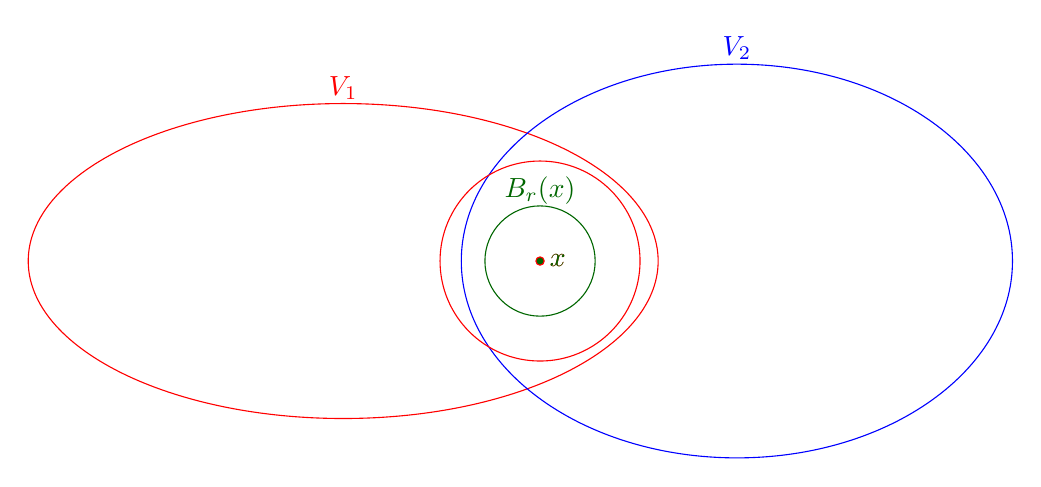
\begin{tikzpicture}
				      \draw[red] (0,0) circle [x radius=4cm, y radius=2cm] ;
				      \draw[blue] (5,0) circle [x radius=3.5cm, y radius=2.5cm] ;
				      \draw (0,2.2) node[red]{$V_1$};
				      \draw (5,2.7) node[blue]{$V_2$};
				      \draw [red] (2.5,0) circle (1.27cm) ;
				      \filldraw[red] (2.5,0) circle (1.5pt) node[anchor=west]{$\bs{x}$};
				      %	\draw [blue] (2.5,0) circle (0.85cm) node [yshift=1cm]{$B_{r}(x)$} ;
				      \draw [green!40!black] (2.5,0) circle (0.7cm) node [yshift=0.9cm]{$B_{r}(x)$} ;
				      \filldraw[green!40!black] (2.5,0) circle (1pt) node[anchor=west]{$x$};
			      \end{tikzpicture}
		      \end{center}
		      As $x\in V_1$ $\exists$ $r_1$ such that $x\in B_{r_1}(x)\subset V_1$. Similarly $x\in V_2$ $\exists$ $r_2$ such that $x\in B_{r_2}(x)\subset V_2$. Take $r=\min\{r_1,r_2\}$. Thus we have $x\in B_r(x)\subset V_1\cap V_2$

	\end{enumerate}
	The second part for closed sets are left as exercise
\end{myproof}

\section{Topological Space}
\dfn{Topological Space}{\label{topological-space}A topological space is a set $X$ together with a collection of subsets of $X$ (i.e. a subset of the power set of $X$) that is closed under taking arbitrary unions and finite intersections. This collection is called a topology on $X$}


\nt{Union means $\bigcup\limits_{\alpha\in I}S_{\alpha}=\{x\in X\mid \exists\ \alpha\text{ s.t. }x\in S_{\alpha}\}$\\
Intersection means $\bigcap\limits_{\alpha\in I}S_{\alpha}=\{x\in X\mid \forall\alpha,\ x\in S_{\alpha}\}$}

\qs{}{  Suppose i have a topological space $X$ under given some topology. Is the entire set open ? And that the empty set is open ?
}\sol If $I=\phi$, $\bigcup\limits_{\alpha\in I}S_{\alpha}=\{x\in X\mid \exists\ \alpha\in I\text{ s.t. }x\in S_{\alpha}\}$  gives $\phi$
and\\ $\bigcap\limits_{\alpha\in I}S_{\alpha}=\{x\in X\mid \forall\alpha\in I,\ x\in S_{\alpha}\}$  gives $X$ because $\forall\ \alpha\in I$ condition is vacuously true for each $x\in X$.
\nt{Intersection of empty families are not defined in set theory. This brings a very important point. In a set theory you have to have a universe. (Set theory have to avoid paradoxes, Russel Paradox) At the beginning you construct a large enough universe and you taking subsets only from that universe. Notice all subsets we are considering here are subsets of $X$ and here we defined how we union and intersection mean. Though it still this asks what our axioms of set theory. So you can change the part of the definition of \hyperref[topological-space]{topological space} like this ``$\dots$with a collection of subsets of $X$ including the empty set and the whole space$\dots$"} (If you don't like this as it is)
\nt{If $S$ is a subset of metric space $X$, then $S$ is itself a metric space and as such open/closed sets as subsets of metric space}
\qs{}{Is there any connection between being open in $X$ and being open in $S$ (Similar question for closed)}

\sol Let $x\in S$. Now, Ball of radius $r$ in $S = S\cap$ Ball of radius $r$ in $X$. Therefore \begin{align*}
	\text{Open Set in } S & =\bigcup \text{ Balls in }S                    \\
	                      & =\bigcup\ (\text{Balls in }X\cap S)            \\
	                      & =\left(\bigcup \text{ Balls in }X\right)\cap S \\
	                      & =\text{Open set }X\cap S
\end{align*}
Part 2 is left as exercise

\cor{}{
	If $S\subset X$ is open in $X$ then a subset $T$ of $S$ is open in $S\iff $ $T$ is open in $X$}

\cor{}{
	If $S\subset X$ is closed in $X$ then a subset $T$ of $S$ is closed in $S\iff $ $T$ is closed in $X$}

\dfn{Subspace of a Topological Space $X$}{For any subset $S$ of a topological space $X$, the collection $S\cap U$, $U$ open in $X$  is called a subspace.}
\qs{}{Prove that subspace of a metric space $X$ defines a topology on $X$}
\wc{}{ If $x\in $ open $V$ then there exists $r>0$ such that $x\in B_r(x)\subset V$
	\begin{center}
		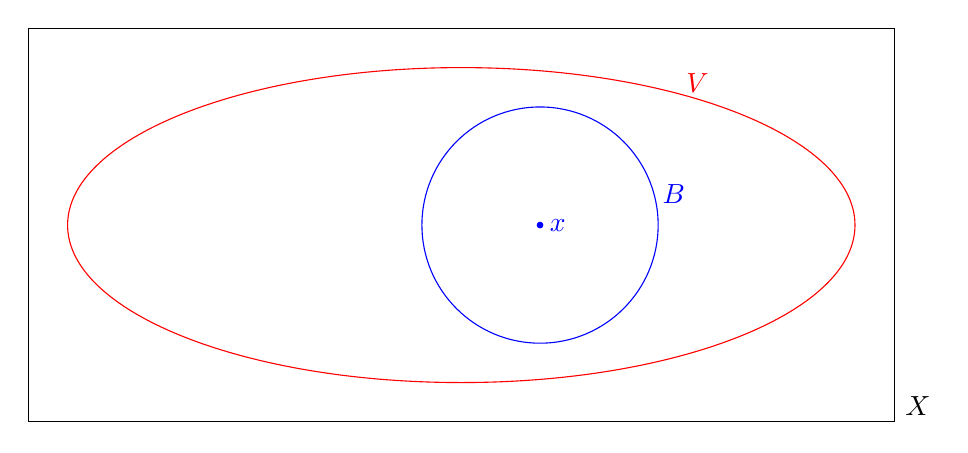
\begin{tikzpicture}
			\draw (-5.5,2.5) rectangle (5.5,-2.5) node[xshift=3mm,yshift=2mm]{$X$};
			\draw[red] (0,0) circle [x radius=5cm, y radius=2cm] ;
			\draw (3,1.8) node[red]{$V$};
			\draw [blue] (1,0) circle (1.5cm) ;
			\filldraw[blue] (1,0) circle (1pt) node[anchor=west]{$x$};
			\draw (2.7,0.4) node[blue]{$B$};
			%\node[black,text width=10cm] at (9,1){If $N$ itseld is open. then we say that $N$ is an open neighbourhood of $x$};
		\end{tikzpicture}
	\end{center}
	\textbf{Idea: }Why not we take $r=\inf \{\text{distance from }x\text{ to boundary of ball } B\}$.

	Now we first have to ensure $r>0$. Suppose that's true.

	Then we have to define boundary. What is boundary, We can give a reasonable definition (Boundary has already a definition but we don't know that for now). Let boundary of $B=\{x\in X\mid d(c,x)=\delta\}$ Now this definition is not proper for our purpose.Because if we take union of all balls in $V$ then we will have lots of points as boundary but part of them should not be considered as boundary. Even if we take this definition.

	Then the big question comes/ We are taking a infimum of a certain set of real numbers. The very first question arises is whether this set is nonempty. For example if we take $B$ to be the metric space it self we have no boundary.
	\tcblower
	Questions which come thorough this.
	\begin{itemize}
		\item Is there a meaningful way to define boundary
		\item Can we modify the idea
	\end{itemize}
}
